\documentclass[11pt]{article}

\usepackage[margin=1in]{geometry}
\usepackage{amsmath,amssymb}
\usepackage{booktabs}
\usepackage{enumitem}
\usepackage{tikz}
\usetikzlibrary{arrows.meta,positioning}
\usepackage{hyperref}

\newcommand{\E}{\mathbb{E}}

\title{Belief-Based Robust Cooperative MARL:\\Context, the Game, and the EIR-MAPPO Algorithm}
\author{Andres Ho}
\date{\today}

\begin{document}
\maketitle

% ============================================================
\section{Context}
% ============================================================

In cooperative multi-agent reinforcement learning (c-MARL), a team of agents shares a
single reward and must learn to coordinate. Most methods assume that every teammate
follows the learned cooperative policy. In practice an agent can be compromised
(hacked or faulty) and act against the team, a \emph{Byzantine} failure. The difficulty
is that nobody knows \emph{which} agent is compromised.

There are three ways to respond:
\begin{enumerate}
  \item \textbf{Ignore it.} A single bad agent can collapse the team. Under a worst-case
        attack on the toy game below, standard MAPPO obtains 4.75 out of a possible 50
        per episode.
  \item \textbf{Assume everyone might be bad} (\emph{ex ante} robustness). This is robust
        but pessimistic: cooperation suffers even when nobody is compromised.
  \item \textbf{Infer who is bad, then act on it} (\emph{ex interim} robustness). Each agent
        keeps a \emph{belief} about its teammates and defends only when the evidence
        supports it.
\end{enumerate}
This work builds on the third approach, introduced by Li et al.\ (ICLR 2024),
\emph{Byzantine Robust Cooperative Multi-Agent Reinforcement Learning as a Bayesian Game},
and their algorithm EIR-MAPPO.

% ============================================================
\section{The game}
% ============================================================

\subsection{The toy game}
We use the toy coordination game of Han et al.\ (2022), also used by Li et al. There are
two agents, two actions $\{0,1\}$ per agent, and two states. Both agents observe the state,
and each episode lasts 100 steps.

\begin{itemize}
  \item In state $s_0$ (XNOR) the team receives reward 1 if the agents \textbf{agree}.
  \item In state $s_1$ (XOR) the team receives reward 1 if the agents \textbf{differ}.
  \item Agreeing flips the state; differing keeps it (Figure~\ref{fig:toy}).
\end{itemize}

\begin{figure}[h]
  \centering
  \begin{minipage}{0.45\textwidth}
    \centering
    \begin{tabular}{c|cc}
      $s_0$ & $0$ & $1$ \\ \hline
      $0$ & 1 & 0 \\
      $1$ & 0 & 1
    \end{tabular}
    \hspace{1.5em}
    \begin{tabular}{c|cc}
      $s_1$ & $0$ & $1$ \\ \hline
      $0$ & 0 & 1 \\
      $1$ & 1 & 0
    \end{tabular}
  \end{minipage}
  \begin{minipage}{0.45\textwidth}
    \centering
    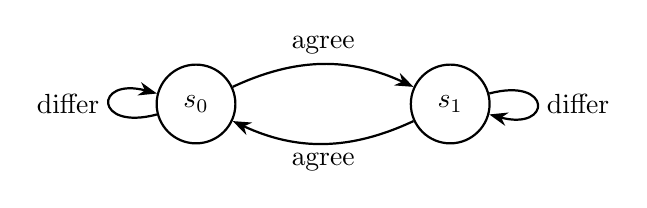
\begin{tikzpicture}[st/.style={circle,draw,thick,minimum size=1cm}, >=Stealth]
      \node[st] (s0) {$s_0$};
      \node[st,right=2.2cm of s0] (s1) {$s_1$};
      \draw[->,thick] (s0) to[bend left=25] node[above] {agree} (s1);
      \draw[->,thick] (s1) to[bend left=25] node[below] {agree} (s0);
      \draw[->,thick] (s0) to[loop left] node[left] {differ} (s0);
      \draw[->,thick] (s1) to[loop right] node[right] {differ} (s1);
    \end{tikzpicture}
  \end{minipage}
  \caption{Left: shared reward in each state (rows: agent 1's action, columns: agent 2's
  action). Right: state transitions.}
  \label{fig:toy}
\end{figure}

\paragraph{Clean play.} Without an adversary, the optimal strategy is to agree in $s_0$ and
differ in $s_1$, which earns reward 1 per step (100 per episode). Differing in $s_1$
requires the two agents to take different roles.

\paragraph{Play under attack.} If one agent is the adversary, the game becomes
\emph{matching pennies}: the honest agent wants to match (in $s_0$) or mismatch (in $s_1$)
the adversary, and the adversary wants the opposite. Any predictable strategy is exploited
and its reward drops toward 0. The best defense is to play each action with probability
$1/2$, which guarantees an expected reward of $0.5$ per step (50 per episode).
Robustness in this game therefore means: coordinate when the partner is honest, and
randomize exactly when the partner is the adversary. This requires knowing \emph{who} the
adversary is.

\subsection{The Bayesian game}
\begin{itemize}
  \item \textbf{Hidden types.} Each agent has a type $\theta^i \in \{0,1\}$, where $1$ means
        compromised. Types are drawn at the start of each episode, stay fixed for the
        episode, and are not observed by the other agents.
  \item \textbf{Prior.} Kept fixed during training:
        \[
          p(\theta = \mathbf{0}) = 0.5, \qquad
          p(\theta = \mathbf{1}_i) = \frac{0.5}{N} \quad \text{for each agent } i.
        \]
        Half of the episodes are clean, and the other half have exactly one adversary.
  \item \textbf{Corruption.} The action executed for agent $i$ is
        \[
          \bar a^i =
          \begin{cases}
            \hat a^i & \text{(the adversary's action) if } \theta^i = 1,\\
            a^i & \text{(the team's action) if } \theta^i = 0.
          \end{cases}
        \]
  \item \textbf{Belief.} Each agent infers the types from its history
        $H^i_t$ of observations and actions:
        \[
          b^i_t = p(\theta \mid H^i_t).
        \]
\end{itemize}

\subsection{Solution concept}
Li et al.\ define an \emph{ex interim robust equilibrium}:
\begin{itemize}
  \item each cooperative agent best-responds given its \textbf{belief},
  \item the adversary best-responds to the team in the worst case, i.e.\ it minimizes the
        team's reward,
  \item beliefs are consistent with Bayes' rule.
\end{itemize}
Informally,
\[
  \max_{\text{team}} \ \min_{\text{adversary}} \ \E_{\theta \sim b}\big[\text{team return}\big].
\]
This is a \emph{saddle point}: the team maximizes and the adversary minimizes the same
quantity, so training has two players pulling in opposite directions.

% ============================================================
\section{The EIR-MAPPO algorithm}
% ============================================================

\subsection{The four networks}

\begin{table}[h]
  \centering
  \begin{tabular}{@{}llll@{}}
    \toprule
    Network & Input & Output & Kept at test time \\
    \midrule
    Team policy $\pi_\phi$ & observation, belief, agent ID & action probabilities & yes \\
    Adversary $\hat\pi_{\hat\phi}$ & observation, agent ID & action probabilities & no \\
    Critic $V_\psi$ & observation, belief & expected future reward & no \\
    Belief $p_\xi$ (GRU) & history of observations & P(each agent is the adversary) & yes \\
    \bottomrule
  \end{tabular}
  \caption{Networks used by EIR-MAPPO.}
\end{table}

One team network is shared by all agents; the agent ID lets the agents take different
roles. The critic and the adversary are only used during training.

\subsection{One training iteration}
Each iteration consists of the following blocks. Blocks 3--6 all use the batch collected
in Block 1, and Block 7 decides which of them run.

\paragraph{Block 1: Play (rollout).}
The current networks play 10 parallel games for 200 steps. At every step, for every agent
$i$:
\begin{enumerate}[nosep]
  \item the belief is updated, $b^i_t = p_\xi(\theta \mid H^i_t)$;
  \item the team proposes an action $a^i_t \sim \pi_\phi(\cdot \mid o^i_t, b^i_t)$;
  \item the adversary proposes an action $\hat a^i_t \sim \hat\pi_{\hat\phi}(\cdot \mid o^i_t)$;
  \item the compromised agent's action is replaced: $\hat a^i_t$ is executed if
        $\theta^i = 1$, otherwise $a^i_t$;
  \item the game returns a shared reward $r_t$ and the next state.
\end{enumerate}
Observations, beliefs, actions, rewards and the true types $\theta$ are stored.

\paragraph{Block 2: Score the actions (advantage).}
For every step the algorithm computes whether the outcome was better or worse than the
critic expected, using generalized advantage estimation (GAE):
\[
  \delta_t = r_t + \gamma\, V_\psi(s_{t+1}) - V_\psi(s_t),
  \qquad
  A_t = \sum_{l \ge 0} (\gamma\lambda)^l\, \delta_{t+l},
\]
with $\gamma = 0.99$ and $\lambda = 0.95$. Here $\delta_t$ is the one-step surprise
(reward received minus reward expected), and $A_t$ averages it over the following steps:
$A_t > 0$ means better than expected, $A_t < 0$ worse. Because the critic is conditioned on
the belief, $A_t$ measures ``better than expected given what the agent believes.'' The same
$A_t$ is used by the team (Block 3) and the adversary (Block 4).

\paragraph{Block 3: Update the team.}
The team should do more of the actions that scored well and less of the others. Only the
steps where the agent was honest ($\theta^i = 0$) are used:
\[
  \max_\phi \ \E\big[(1-\theta^i)\,\log \pi_\phi(a^i_t \mid o^i_t, b^i_t)\; A_t\big].
\]
In practice this is optimized with PPO: the probability of an action may change by at most
about 5\% per update (clip $=0.05$), an entropy bonus ($0.01$) keeps the policy exploring,
and the batch is used for 5 passes (epochs).

\paragraph{Block 4: Update the adversary.}
The adversary uses the same rule with the sign flipped: it does more of whatever
\emph{hurt} the team. Only the steps where the agent was compromised ($\theta^i = 1$) are
used:
\[
  \max_{\hat\phi} \ \E\big[\theta^i\, \log \hat\pi_{\hat\phi}(\hat a^i_t \mid o^i_t)\; (-A_t)\big],
\]
with the same PPO settings as the team. The team needs a strong attacker to train against
in order to become robust.

\paragraph{Block 5: Update the critic.}
The critic is trained to predict the discounted reward that actually followed:
\[
  \min_\psi \ \E\Big[\big(V_\psi(o^i_t, b^i_t) - \text{return}_t\big)^2\Big].
\]
In practice a Huber loss is used, targets are normalized (PopArt), and the change in the
predicted value per update is limited. A better critic gives better advantages in Block 2,
and therefore better updates for both players.

\paragraph{Block 6: Update the belief.}
The belief network (a GRU over the agent's history) is trained with the true types, which
are known during training, using binary cross-entropy:
\[
  \min_\xi \ \E\Big[-\theta \log p_\xi(\theta \mid H^i_t)
    - (1-\theta)\log\big(1 - p_\xi(\theta \mid H^i_t)\big)\Big].
\]
The best possible predictor under this loss is the true posterior $P(\theta \mid H)$, so the
network learns Bayes-consistent beliefs without ever computing Bayes' rule explicitly.

\paragraph{Block 7: The schedule (two timescales).}
The adversary is updated on every iteration, while the team, critic and belief are updated
only on every 10th iteration:

\begin{table}[h]
  \centering
  \begin{tabular}{@{}lcc@{}}
    \toprule
    Iteration $k$ & Adversary (Block 4) & Team, critic, belief (Blocks 3, 5, 6) \\
    \midrule
    $k \bmod 10 \neq 0$ & update & frozen \\
    $k \bmod 10 = 0$ & update & update \\
    \bottomrule
  \end{tabular}
  \caption{Two-timescale schedule.}
\end{table}

The adversary therefore stays close to the strongest attack, and the team always trains
against a near worst case; this is the basis of the paper's convergence argument. The
learning rates are equal for both players, and the different timescales come from the
update frequency (the authors report that faster adversary learning rates were unstable).
In practice, however, the two players can still chase each other in circles, as is typical
of matching pennies. This is the motivation for our method.

\subsection{Summary of the training loop}
\begin{enumerate}[nosep]
  \item \textbf{Play:} collect episodes with the current networks.
  \item \textbf{Score:} was each step better or worse than expected?
  \item \textbf{Team:} do more of what helped.
  \item \textbf{Adversary:} do more of what hurt.
  \item \textbf{Critic:} predict rewards better.
  \item \textbf{Belief:} guess the compromised agent better.
  \item \textbf{Schedule:} the adversary every iteration, the rest every 10th.
\end{enumerate}

\subsection{Evaluation protocol}
Robustness is measured as follows:
\begin{enumerate}[nosep]
  \item the team is trained with 5 random seeds;
  \item for each seed and each agent $i$, the team (policy and belief) is frozen and a fresh
        PPO adversary that always controls agent $i$ is trained against it;
  \item the team's reward per episode under that attack is recorded;
  \item the result is the mean over the $5 \times N$ attacks.
\end{enumerate}
On the toy game, EIR-MAPPO obtains \textbf{44.14} out of a maximum of 50 per episode under
this worst-case attack (Fig.~6 of the paper).

\subsection{Hyperparameters}

\begin{table}[h]
  \centering
  \begin{tabular}{@{}llll@{}}
    \toprule
    Parameter & Value & Parameter & Value \\
    \midrule
    parallel rollouts & 10 & rollout length & 200 \\
    PPO epochs & 5 & PPO clip & 0.05 \\
    discount $\gamma$ & 0.99 & GAE $\lambda$ & 0.95 \\
    entropy coefficient & 0.01 & max gradient norm & 10 \\
    learning rates (all) & $5\times10^{-5}$ & optimizer & Adam \\
    hidden size & 128 & belief network & GRU \\
    value normalization & PopArt & critic loss & Huber ($\delta = 10$) \\
    adversary interval & 10 & output layer gain & 0.01 \\
    \bottomrule
  \end{tabular}
  \caption{EIR-MAPPO hyperparameters for the toy game (Table 1 of the paper).}
\end{table}

\end{document}
